\documentclass[conference]{IEEEtran}
\usepackage{graphicx}
\usepackage{booktabs}
\usepackage{url}
\title{A Reproducibility and Transportability Audit of Cardiovascular Prediction Under Dataset Shift}
\author{\IEEEauthorblockN{Akhil Preetham E, Ch Hari Krishna, and G Vennela}
\IEEEauthorblockA{Department of Computer Science and Engineering\\
Prasad V. Potluri Siddhartha Institute of Technology, Vijayawada, India\\
\textit{Working draft; author order, contributions, and affiliations require confirmation before submission}}}
\begin{document}
\maketitle

\begin{abstract}
High discrimination on small public cardiovascular datasets can obscure leakage, uncertain endpoint provenance, poor calibration, and weak performance after transport. We report a reproducibility and transportability audit of CARDIODIAG, a tabular coronary artery disease (CAD) prediction project. We first corrected the internal evaluation boundary and repeated nested model selection on two historical benchmarks. Corrected optimized voting achieved mean outer-fold ROC-AUC 0.930 (SD 0.007) on a 918-row derived ``Five States'' composite and 0.996 (SD 0.001) on the 2021 Mendeley benchmark. These results are internal benchmark estimates; the latter dataset lacks a documented diagnostic reference standard and prediction time, and the former has unresolved upstream provenance and reuse terms. A stability-aware feature selector did not show a clear advantage over one-shot selection. Across ten internal fit/calibration/evaluation splits, nominal 90\% split-conformal sets achieved empirical coverage of 0.906--0.909, while calibration error depended strongly on whether bins were macro-averaged or weighted by sample count. Source-only transfer stress tests were substantially less reassuring: ROC-AUC was 0.720 on Z-Alizadeh Sani, 0.787 on AngioCAD, and 0.661 on Duke ACATH, whose stenosis threshold differs from the source. Feature-only out-of-distribution separation was weak (AUROC 0.58--0.60). A combined conformal and support rule accepted only 21 of 377 AngioCAD records (5.6\%), all positive; the apparent absence of errors is therefore uninformative about safety. The results support a reproducible research prototype, but do not establish clinically useful transportability, reliable shift detection, or clinical readiness.
\end{abstract}
\begin{IEEEkeywords}
cardiovascular disease, coronary artery disease, dataset shift, calibration, conformal prediction, external evaluation, reproducibility
\end{IEEEkeywords}

\section{Introduction}
Machine-learning studies of cardiovascular disease often report high internal discrimination on small, reused benchmark datasets. Such estimates can be optimistic when feature selection or model selection sees evaluation data, and they do not by themselves establish probability calibration, utility at a clinical operating point, or performance at a new hospital. These issues are central to clinical prediction reporting and risk-of-bias assessment \cite{collins2024tripodai,moons2025probastai}. External cardiovascular model evaluations have also documented that performance varies across settings \cite{wessler2021external}.

CARDIODIAG began as an implementation of feature reduction and ensemble prediction for heart-disease classification \cite{khan2026cardiodiag}. Its inherited benchmarks produced strong scores, but a source and code audit identified evaluation-boundary defects and unresolved data semantics. We therefore reframed the work as a reproducibility and transportability audit rather than a claim of a new clinically validated algorithm. We ask: (1) what performance remains after nested, training-only preprocessing and selection; (2) does repeated feature selection improve stability or reliability; and (3) do source-calibrated predictions, out-of-distribution (OOD) warnings, and abstention remain useful on separately reported cohorts?

The main contribution is an evidence-constrained evaluation across corrected internal experiments and three site-level transport stress tests. The results include negative findings: two internal benchmarks remain easy to discriminate, but they do not resolve endpoint validity; feature-only OOD detection is weak; and selective prediction either has very low coverage or retains material error. We distinguish these results from verified independent external validation and identify data-rights and protocol limits that must be resolved before submission or release.

\section{Data and Study Design}
\subsection{Internal benchmarks}
The Five States benchmark contains 918 labelled rows. An audit maps the rows to UCI Heart Disease components, with 914 unique matches and four ambiguous matches due to source missingness. The exact upstream composite, version, transformation history, and standalone reuse terms were not recovered. It is not independent of its UCI components. The 2021 Mendeley cardiovascular dataset has a declared CC BY 4.0 license, but its codebook does not provide an angiographic reference standard, stenosis threshold, or predictor index time \cite{doppala2021dataset}. Neither benchmark establishes prospective pre-diagnostic performance. The later 2026 Mendeley release was used only for provenance screening: all 918 labelled rows exactly match Five States \cite{mendeleyheart2026}.

The UCI source cohorts (Cleveland, Hungary, Switzerland, and VA Long Beach; 920 records total) were used for a retrospective source-domain pilot. These records overlap the Five States composite. Statlog was excluded as a new cohort because all 270 records match Cleveland after label harmonization \cite{ucihd,ucistatlog}. Consequently, the apparent number of data files is larger than the number of independent patient cohorts. We treat the UCI-derived benchmarks as repeated views of related source data, not as independent replications.

\subsection{Transport stress-test cohorts}
The Z-Alizadeh Sani cohort contains 303 patients reported from a Tehran hospital, including 216 CAD and 87 normal labels \cite{alizadehsani2013cad,uciz}. The model used age, sex, and fasting-glucose status; the target is stenosis $\geq 50\%$, whereas the UCI source target uses $>50\%$. Public records lack identifiers for overlap checks.

AngioCAD reports 413 labelled IDs from an Isfahan hospital; 377 have matching clinical feature rows. Its target was derived from 15 artery-segment categories as stenosis $>50\%$ \cite{angiocad2026,angiocadzenodo2025}. The released bins do not isolate exact 50\% cases, age and fasting-glucose units are undocumented, and 36 labelled IDs lack matched feature rows for unknown reasons. The cohort is separately reported, but person-level independence from source data cannot be verified. Outcomes were examined before the subsequent reliability replay, so that replay is post hoc.

Duke ACATH contains 3,504 records; its significant-disease endpoint begins at $\geq 75\%$ stenosis, and cholesterol is missing for 1,246 records \cite{dukeacath2026}. The provider permits use with attribution, but standardized redistribution terms are unspecified. Duke is an endpoint-mismatched stress test, not a same-endpoint validation cohort. No new controlled-access clinical cohort was acquired for this study.

\subsection{Evaluation protocols}
We retain three evidence classes: corrected internal nested validation, internal reliability/stability experiments, and source-only transfer stress tests. They are not pooled. Internal nested runs used three outer folds, three inner folds, and seed 42. Preprocessing, feature selection, hyperparameter choice, and out-of-fold stacking were confined to each outer training partition; each outer test fold was scored once. We report fold-mean ROC-AUC and secondary precision-recall area (PR-AUC), Brier score, and expected calibration error (ECE). Descriptive intervals over folds are not patient-level confidence intervals.

For stability, five stratified folds were repeated three times. A repeated training-only relevance selector was compared with a one-shot selector using the chance-corrected Nogueira stability statistic \cite{nogueira2018stability}. For internal selective reliability, ten seeds (42--51) used disjoint 56.25\% fit, 18.75\% calibration, and 25\% evaluation partitions. No evaluation labels were used for model fitting or calibration. For transfer, source training used the four UCI cohorts with equal total fitting weight per cohort. The Z-Alizadeh Sani and initial AngioCAD transfer used age, sex, and fasting-glucose status and source-only Platt calibration. Subsequent reliability experiments used disjoint 70\% fit, 15\% probability-calibration, and 15\% conformal/OOD-calibration source partitions. Duke used age, sex, and cholesterol.

\begin{figure*}[t]
\centering
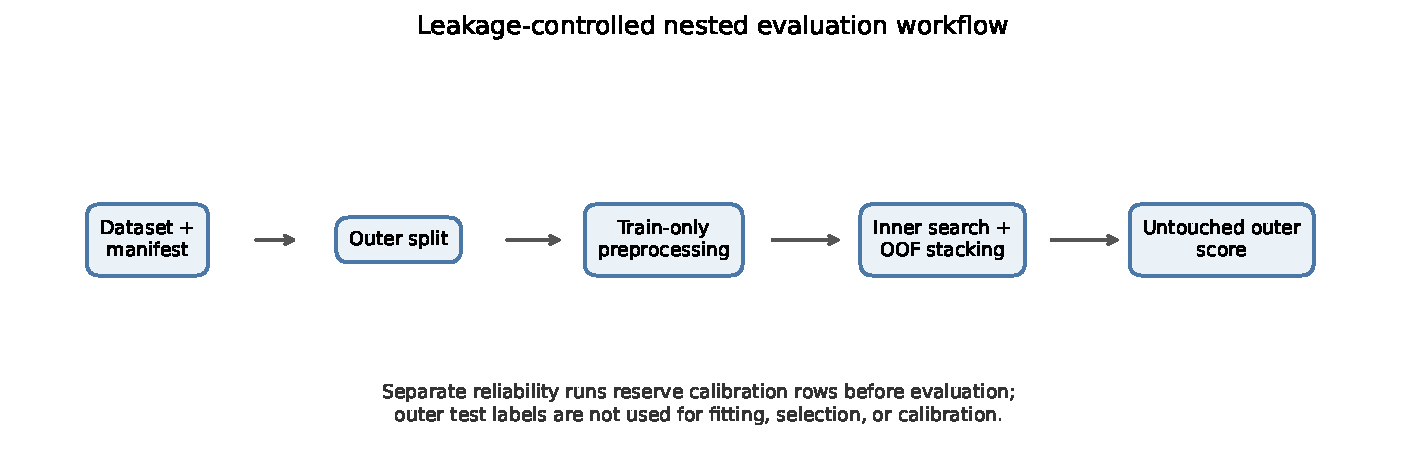
\includegraphics[width=0.92\textwidth]{figures/research_workflow.pdf}
\caption{Evaluation boundary used in the corrected internal experiments. All data-dependent selection is fit within the training side of each outer split. Separate source calibration partitions are reserved for probability calibration and uncertainty thresholds.}
\label{fig:workflow}
\end{figure*}

\section{Methods}
\subsection{Leakage-controlled model evaluation}
The corrected pipeline uses fold-fitted imputation, categorical encoding, and numeric preprocessing. Identifiers are excluded. Candidate classifiers and ensemble weights are selected within inner folds; the outer test partition is not used to select a model. Internal performance estimates are reported as benchmark discrimination and calibration, not as evidence of deployment performance. The distinction matters because model selection on reused validation data can bias error estimates \cite{varma2006bias,cawley2010overfitting}.

The stability-aware selector estimates feature relevance across training-only perturbations, retains predictors meeting prespecified frequency and relevance thresholds, and is compared with one-shot relevance selection. Its purpose is to assess repeatability, not causal feature importance. The stability statistic is calculated over repeated selections; bootstrap intervals summarize the three repeat-level differences and are consequently descriptive and imprecise.

\subsection{Calibration, conformal sets, and selective prediction}
We report Brier score and ten-bin calibration errors. Macro-bin ECE gives equal weight to each occupied bin; weighted ECE weights by the fraction of observations in each bin. These summaries can differ markedly when bins have different sizes, so we report both. Calibration is a separate property from ranking performance \cite{vancalster2019calibration}.

Binary split-conformal sets were constructed from source-calibrated nonconformity scores $1-p(y)$ using the maximum per-source finite-sample 90\% quantile. Empirical coverage is assessed on evaluation data. Its nominal guarantee relies on exchangeability and does not automatically carry across dataset shift \cite{angelopoulos2023conformal}. OOD comparators include Isolation Forest and a 10-nearest-neighbor feature-support distance, thresholded from source calibration data. For the latter, the score is mean Euclidean distance to ten source-fitting neighbors and the threshold is the 95th percentile of source-calibration scores. The Isolation Forest comparator is likewise fit and thresholded without target labels. A combined selective output required a singleton conformal set and feature-support score within the source threshold. A metadata gate abstained when the supplied site identifier was absent from the registered source domains; this uses trusted provenance metadata and is not learned OOD detection. These layers answer different questions: the conformal set represents label uncertainty under source exchangeability, the support score flags feature-space distance, and the site gate enforces a declared operating boundary.

External bootstrap intervals use 1,000 class-stratified resamples and condition on observed class counts. AngioCAD's later conformal/support and risk--coverage replays are explicitly post hoc. Target labels were used only to score the frozen external predictions and were never used to fit the source model or thresholds. This conditioning gives a descriptive interval for the observed case mix; it does not account for uncertainty in prevalence, site selection, data linkage, or between-hospital variation. Confidence-error AUROC measures whether model confidence ranks correct predictions above errors; it is not a calibrated probability of correctness. AURC was computed as the arithmetic mean of cumulative error risks over retained-prefix sizes, so comparisons with studies using numerical integration require caution.

\section{Results}
\subsection{Internal discrimination and calibration}
Corrected optimized voting (OVEC) had the highest mean outer-fold ROC-AUC among the listed candidates on both benchmarks: 0.930 (SD 0.007) on Five States and 0.996 (SD 0.001) on Mendeley (Table~\ref{tab:internal}). Its PR-AUC values were 0.933 and 0.997, respectively. The Brier score was 0.100 and 0.025, while the legacy macro-bin ECE was 0.086 and 0.158. Thus discrimination was high, but calibration was not uniformly low, particularly on the Mendeley benchmark. The Mendeley benchmark's undocumented outcome and predictor timing limit clinical interpretation even if the internal separation is reproducible.

\begin{table}[t]
\centering
\caption{Corrected nested internal results for optimized voting. Fold summaries are internal benchmark evidence, not external validation.}
\label{tab:internal}
\footnotesize
\resizebox{\columnwidth}{!}{\begin{tabular}{lrrrr}
\toprule
Benchmark & ROC-AUC (SD) & PR-AUC & Brier & Macro ECE\\
\midrule
Five States ($n=918$) & 0.930 (0.007) & 0.933 & 0.100 & 0.086\\
Mendeley 2021 & 0.996 (0.001) & 0.997 & 0.025 & 0.158\\
\bottomrule
\end{tabular}}
\end{table}

\subsection{Feature stability and internal selective reliability}
Stable-minus-one-shot Nogueira stability differences were 0.097 (95\% descriptive bootstrap interval $[-0.027,0.198]$) on Five States and 0.069 ($[0.000,0.167]$) on Mendeley. The uncertainty intervals touch or cross zero, and each is based on only three repeat-level differences. We therefore find no decisive evidence that the repeated selector improves stability. Nor did the stability analysis establish a predictive or reliability advantage.

Across ten internal fit/calibration/evaluation seeds, corrected and stable OSEC achieved empirical 90\% conformal coverage of 0.908/0.909 on Five States and 0.906/0.908 on Mendeley (Table~\ref{tab:reliability}). Macro-bin ECE was 0.121 and 0.221 for corrected OSEC; weighted ECE was 0.062 and 0.031. This large convention-dependent difference is a warning against presenting ECE without its definition. Confidence-error AUROC was 0.761 on Five States and 0.905 on Mendeley for corrected OSEC. The corresponding AURC values were 0.0505 and 0.0041; stable OSEC did not improve them (0.0516 and 0.0042). AURC follows the retained-prefix arithmetic-mean convention described above. These internal summaries do not show performance under external shift.

\begin{table}[t]
\centering
\caption{Ten-seed internal selective reliability. Coverage is empirical evaluation-partition coverage; ECE definitions differ by bin weighting.}
\label{tab:reliability}
\footnotesize
\resizebox{\columnwidth}{!}{\begin{tabular}{lrrrrr}
\toprule
Benchmark/model & Coverage & Conf.-err. AUC & AURC & Macro ECE & Wtd. ECE\\
\midrule
Five States, corrected & 0.908 & 0.761 & 0.0505 & 0.121 & 0.062\\
Five States, stable & 0.909 & 0.760 & 0.0516 & 0.121 & 0.060\\
Mendeley, corrected & 0.906 & 0.905 & 0.0041 & 0.221 & 0.031\\
Mendeley, stable & 0.908 & 0.905 & 0.0042 & 0.217 & 0.029\\
\bottomrule
\end{tabular}}
\end{table}

\begin{figure}[t]
\centering
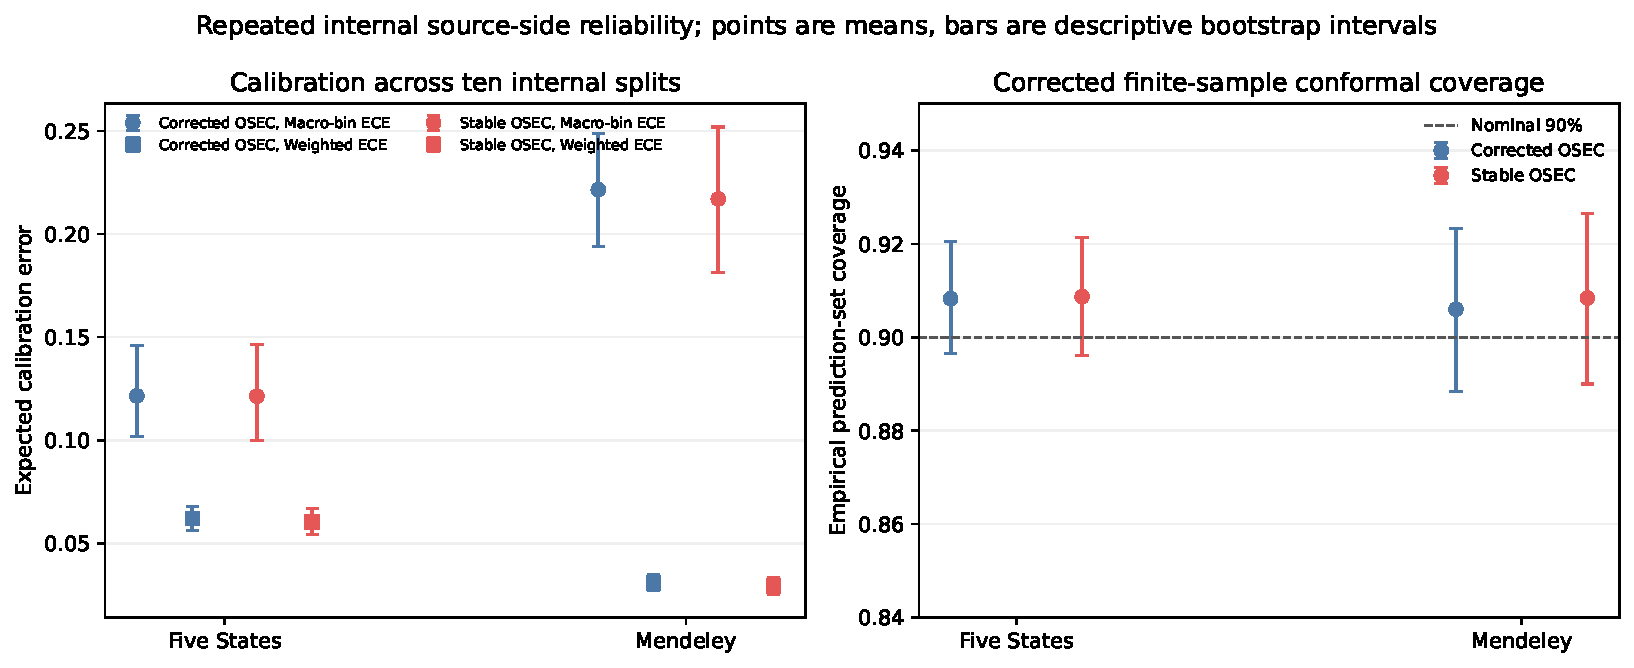
\includegraphics[width=0.98\columnwidth]{figures/corrected_reliability.pdf}
\caption{Internal reliability diagnostics from the corrected repeated evaluation. Nominal conformal coverage is near 90\%; calibration error depends on the bin-weighting convention.}
\label{fig:reliability}
\end{figure}

\subsection{Source-only transfer and OOD analysis}
On Z-Alizadeh Sani, the source-only model achieved ROC-AUC 0.720 (95\% conditional bootstrap CI 0.651--0.780) and average precision 0.853 (0.807--0.894). Platt calibration changed Brier score from 0.200 to 0.193 and ECE from 0.136 to 0.110 by point estimate; paired intervals included no difference. Feature-only OOD AUROC was 0.604 (0.552--0.652); it flagged 14.9\% of target rows at a 5.3\% source false-alert rate. Flagged records had a worse Brier score by point estimate, but this subgroup contained only five negative cases. The warning therefore did not establish reliable individual error detection. The different $\geq 50\%$ target definition and unavailable person identifiers mean this is a transport stress test rather than a verified independent same-endpoint validation.

The initial source-only AngioCAD evaluation achieved ROC-AUC 0.787 (0.734--0.838) and average precision 0.932 (0.913--0.952). Source Platt calibration changed Brier score from 0.190 to 0.185 but increased ten-bin ECE from 0.211 to 0.216; paired intervals included no difference. Isolation Forest source--target AUROC was 0.589 (0.541--0.635), indicating weak separation. A later disjoint-calibration replay yielded ROC-AUC 0.790 (0.733--0.837), but is post hoc because the AngioCAD outcomes had already been inspected. Its kNN OOD AUROC was 0.580 (0.527--0.635).

Duke ACATH achieved ROC-AUC 0.661 (0.642--0.680). Source Platt calibration worsened Brier score from 0.216 to 0.241 and ECE from 0.119 to 0.198. Isolation Forest OOD AUROC was 0.598. Its conformal set covered 98.3\% of Duke records empirically and was singleton for 13.9\%; the combined conformal/support rule made 401 predictions and produced 41 errors among them. Interpretation is further limited by the Duke $\geq 75\%$ outcome versus the source $>50\%$ outcome and extensive missing cholesterol. Across the three target cohorts, feature-only OOD discrimination was weak and did not support reliable automatic shift rejection (Fig.~\ref{fig:ood}).

Table~\ref{tab:external} places the observed target estimates side by side while retaining the endpoint and timing qualifications. These are not three interchangeable replications: the feature sets differ, the positive-label definitions differ, and the later AngioCAD reliability replay uses a target that had already been examined. The combined OOD AUROCs near 0.6 indicate that these scores carry little standalone information for separating source from target in these experiments. An AUROC near 0.5 would be chance ranking; these estimates are only modestly above that reference and their intervals include values close to chance.

\begin{table*}[t]
\centering
\caption{Source-only transfer stress tests. Intervals are conditional class-stratified bootstrap intervals. OOD AUROC is based on feature-space scores, not outcome prediction.}
\label{tab:external}
\footnotesize
\setlength{\tabcolsep}{3pt}
\begin{tabular}{p{0.13\textwidth}r p{0.17\textwidth} p{0.21\textwidth} p{0.12\textwidth} p{0.16\textwidth}}
\toprule
Cohort & $n$ & Target vs. source & ROC-AUC (95\% CI) & OOD AUROC & Main qualification\\
\midrule
Z-Alizadeh Sani & 303 & $\geq 50\%$ vs. $>50\%$ & 0.720 (0.651--0.780) & 0.604 (IF) & Different cutoff; linkage unavailable\\
AngioCAD, initial & 377/413 & Derived $>50\%$ vs. $>50\%$ & 0.787 (0.734--0.838) & 0.589 (IF) & Units undocumented; unmatched IDs\\
AngioCAD, replay & 377/413 & Same target; post hoc & 0.790 (0.733--0.837) & 0.580 (kNN) & Target previously examined\\
Duke ACATH & 3,504 & $\geq 75\%$ vs. $>50\%$ & 0.661 (0.642--0.680) & 0.598 (IF) & Cholesterol missing in 1,246\\
\bottomrule
\end{tabular}
\end{table*}

\begin{figure}[t]
\centering
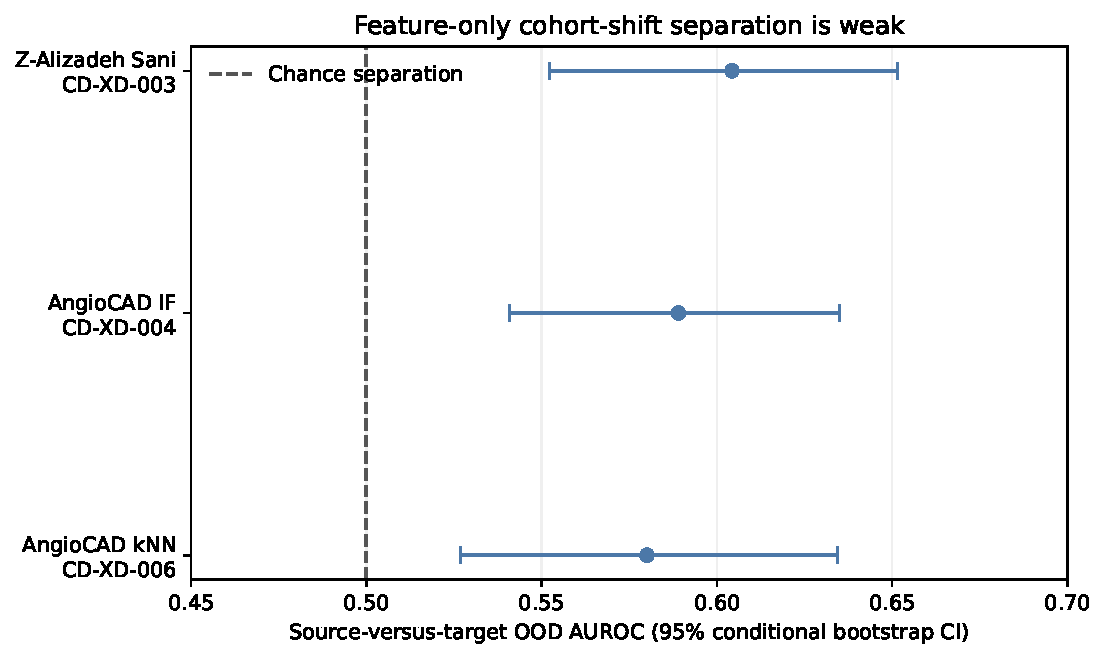
\includegraphics[width=0.98\columnwidth]{figures/ood_separation_summary.pdf}
\caption{Feature-based source--target OOD discrimination was weak on the reported cohorts. Cohort definitions and analysis timing differ; the AngioCAD kNN result is post hoc.}
\label{fig:ood}
\end{figure}

\subsection{Selective prediction and operating coverage}
In the post-hoc AngioCAD replay, source conformal sets covered all 377 target records empirically, but were singleton for only 33 (8.8\%). Requiring both a singleton set and acceptable feature support returned predictions for 21 records (5.6\%). All 21 were positive, with zero observed errors. Since there were no accepted negative cases and coverage was very low, this result cannot establish a useful low-risk operating point. The site metadata gate abstained on all 377 AngioCAD records because the site was unregistered. For Duke, the combined rule accepted 401/3,504 (11.4\%) records and made 41 errors among accepted cases (10.2\%). Risk--coverage curves are descriptive; AngioCAD is post hoc and Duke has a different endpoint (Fig.~\ref{fig:risk}).

\begin{figure}[t]
\centering
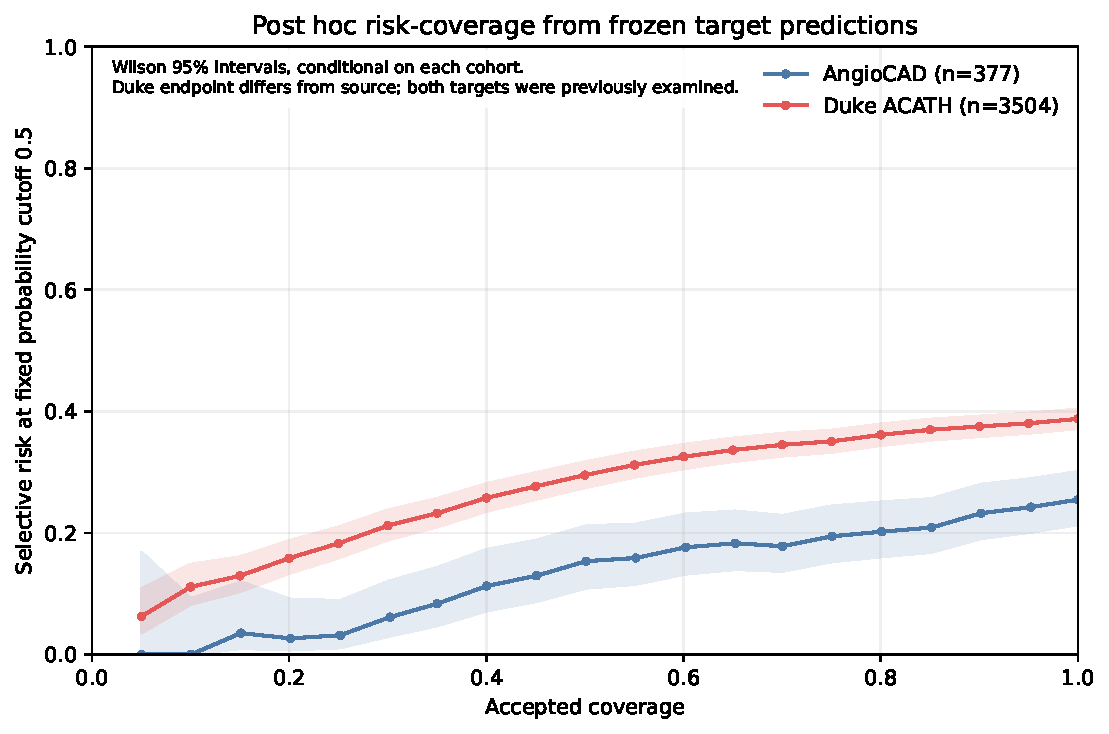
\includegraphics[width=0.98\columnwidth]{figures/posthoc_target_risk_coverage.pdf}
\caption{Post-hoc risk--coverage diagnostics at the frozen probability threshold. Intervals condition on observed cohort class counts; they do not certify safety. AngioCAD outcomes were previously examined, and Duke has an endpoint mismatch.}
\label{fig:risk}
\end{figure}

\section{Discussion}
This audit separates internal benchmark performance from the question that matters for deployment: whether a frozen model remains accurate, calibrated, and useful at a new site. Correcting the evaluation boundary retained strong internal discrimination, but high scores on these reused datasets are not evidence of clinical prediction. The Five States composite has unresolved provenance and reuse terms, while the Mendeley codebook does not establish the clinical endpoint or predictor time. Some inherited predictors may also be downstream of diagnostic testing. These factors can make classification easy without representing prospective risk prediction.

The feature-stability extension did not deliver a clear improvement. The point estimates favored stability-aware selection, but only three repeat-level comparisons were available and the intervals were broad. More fundamentally, repeatable feature sets are not evidence that the selected variables are causal or that the resulting probabilities transport. The ten-seed calibration results show the need to define ECE precisely: a single number can look materially different under macro and sample-weighted binning.

External stress tests weakened the case for generalization. Discrimination ranged from moderate to weak, calibration shifts varied in direction, and OOD detectors separated source and target feature distributions only modestly. A fail-closed site registry can withhold outputs for an unregistered site, but depends on trusted metadata and has zero coverage for a new site by design. Feature-only rejection is not a substitute: the AngioCAD selective rule retained only 5.6\% of cases, all of one class, while the Duke rule retained more cases but had a 10.2\% accepted error fraction. Neither supports a claim of safe or useful selective prediction.

The appropriate project-level conclusion is therefore narrow. CARDIODIAG now provides a reproducible engineering pipeline and a transparent negative transportability result. The available evidence does not support a clinically dependable model, a generalizable feature-selection method, or an effective OOD/abstention method. This is a research no-go for claims of reliable unseen-site prediction, pending evaluation on untouched, endpoint-compatible clinical cohorts. For a next confirmatory study, the target condition and index prediction time should be fixed before data access; source/target inclusion, duplicate detection, missingness, unit mapping, and patient-level splits should be specified; the model and thresholds should be frozen before one-time evaluation; and sample size should be planned for both discrimination and calibration at prespecified operating points. A genuinely new hospital cohort with authorized use and a documented reference standard would address the principal unresolved evidence gap more directly than adding another repackaged benchmark.

\subsection{Limitations and data governance}
All clinical interpretation is limited by retrospective public-data reuse, uncertain predictor timing, endpoint differences, missing measurements, unverified patient-level independence, and small numbers of hospitals. Z-Alizadeh Sani and AngioCAD are not untouched confirmatory cohorts; the AngioCAD reliability and selective analyses are post hoc. The Duke endpoint differs from the source. Bootstrap intervals condition on observed class counts and do not capture between-hospital variation. Conformal coverage under source exchangeability is not a guarantee under shift. The 2026 Mendeley file is a duplicate, not another cohort. The 70,000-row Kaggle cardiovascular dataset has a different target and an unresolved license and is not treated as CAD validation.

The Five States composite is not cleared for redistribution. Raw Duke redistribution terms are unspecified. Raw datasets are excluded from the paper bundle. Before submission, the project team must verify each source's access and attribution conditions, obtain an institutional determination on whether ethics review or exemption applies, and complete funding, competing-interest, and author-contribution declarations. No approval, exemption, external clinical validation, or contribution is invented here.

\section{Conclusion}
Leakage-controlled internal evaluation confirmed strong discrimination on two historical benchmarks, but the provenance and endpoint limitations prevent a clinical claim. Stability-aware selection showed no decisive stability advantage; internal calibration summaries depended on ECE convention; and three source-only transfer stress tests exposed weak OOD separation, mixed calibration, and low-utility selective coverage. CARDIODIAG is a reproducible research prototype, not a clinically ready prediction system. An independent, prospectively specified evaluation on authorized, untouched cohorts with aligned endpoints and recorded prediction timing is required before any clinical utility claim.

\section*{Declarations}
\textbf{Ethics:} Institutional determination pending; no approval or exemption is claimed.\\
\textbf{Funding and competing interests:} Confirmation pending.\\
\textbf{Author contributions:} Contributions require confirmation from all listed authors before submission.\\
\textbf{Data and code availability:} Source datasets are not bundled. Dataset provenance and terms vary; Five States standalone terms and Duke redistribution rights remain unresolved. Code redistribution rights must be confirmed before public release.\\
\textbf{Manuscript status:} Working draft; author order, affiliations, declarations, and venue formatting require review.

\bibliographystyle{IEEEtran}
\bibliography{references}
\end{document}
